\documentclass{standalone}
\usepackage{tikz}
\usetikzlibrary{patterns, positioning}
\usepackage[sfdefault]{ClearSans} %% option 'sfdefault' activates Clear Sans as the default text font
\usepackage[T1]{fontenc}

\begin{document}
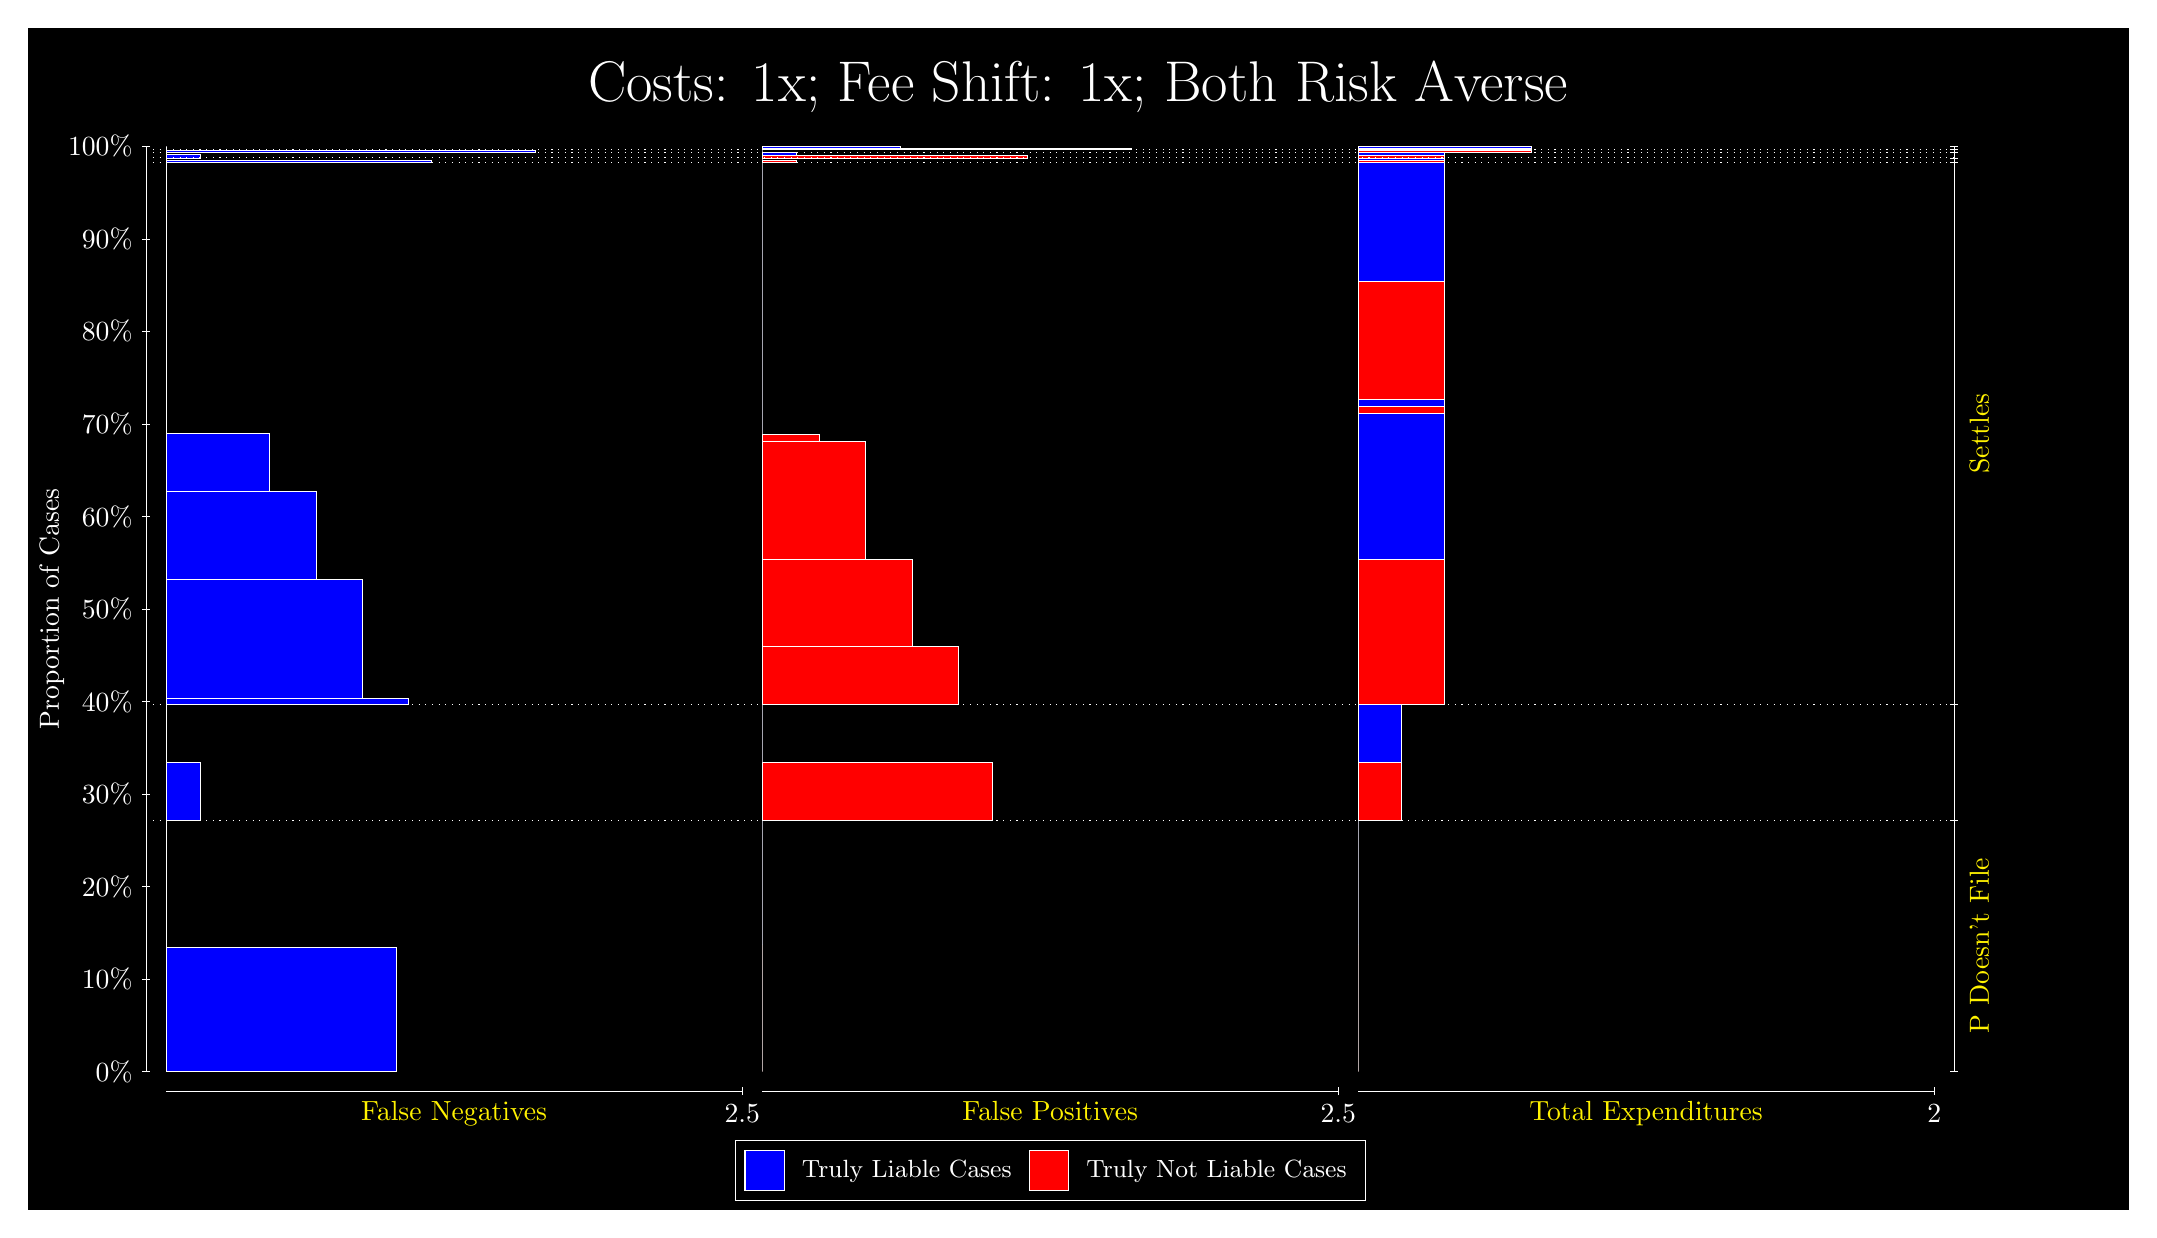
\begin{tikzpicture}
\draw[fill=black] (0,0) rectangle (26.667,15);
\draw[text=white] (0,13.5) rectangle (26.667,15) node[midway] {\huge Costs: 1x; Fee Shift: 1x; Both Risk Averse};
\draw[white, very thin] (1.5,1.75) -- (1.5,13.5);
\node[rotate=90, text=white, anchor=center] at (0.3, 7.625) {Proportion of Cases};
\draw[white, very thin] (1.45,1.75) -- (1.55,1.75);
\node[text=white, anchor=east] at (1.45, 1.75) {0\%};
\draw[white, very thin] (1.45,2.925) -- (1.55,2.925);
\node[text=white, anchor=east] at (1.45, 2.925) {10\%};
\draw[white, very thin] (1.45,4.1) -- (1.55,4.1);
\node[text=white, anchor=east] at (1.45, 4.1) {20\%};
\draw[white, very thin] (1.45,5.275) -- (1.55,5.275);
\node[text=white, anchor=east] at (1.45, 5.275) {30\%};
\draw[white, very thin] (1.45,6.45) -- (1.55,6.45);
\node[text=white, anchor=east] at (1.45, 6.45) {40\%};
\draw[white, very thin] (1.45,7.625) -- (1.55,7.625);
\node[text=white, anchor=east] at (1.45, 7.625) {50\%};
\draw[white, very thin] (1.45,8.8) -- (1.55,8.8);
\node[text=white, anchor=east] at (1.45, 8.8) {60\%};
\draw[white, very thin] (1.45,9.975) -- (1.55,9.975);
\node[text=white, anchor=east] at (1.45, 9.975) {70\%};
\draw[white, very thin] (1.45,11.15) -- (1.55,11.15);
\node[text=white, anchor=east] at (1.45, 11.15) {80\%};
\draw[white, very thin] (1.45,12.325) -- (1.55,12.325);
\node[text=white, anchor=east] at (1.45, 12.325) {90\%};
\draw[white, very thin] (1.45,13.5) -- (1.55,13.5);
\node[text=white, anchor=east] at (1.45, 13.5) {100\%};

\draw[white, very thin] (24.457,1.75) -- (24.457,13.5);
\draw[white, very thin] (24.407,1.75) -- (24.507,1.75);
\node[anchor=west] at (24.407, 1.75) {};
\draw[white, very thin] (24.407,4.9434) -- (24.507,4.9434);
\node[anchor=west] at (24.407, 4.9434) {};
\draw[white, very thin] (24.407,6.4122) -- (24.507,6.4122);
\node[anchor=west] at (24.407, 6.4122) {};
\draw[white, very thin] (24.407,13.292) -- (24.507,13.292);
\node[anchor=west] at (24.407, 13.292) {};
\draw[white, very thin] (24.407,13.353) -- (24.507,13.353);
\node[anchor=west] at (24.407, 13.353) {};
\draw[white, very thin] (24.407,13.427) -- (24.507,13.427);
\node[anchor=west] at (24.407, 13.427) {};
\draw[white, very thin] (24.407,13.463) -- (24.507,13.463);
\node[anchor=west] at (24.407, 13.463) {};
\draw[white, very thin] (24.407,13.5) -- (24.507,13.5);
\node[anchor=west] at (24.407, 13.5) {};

\draw[white, very thin, fill=blue] (1.75,1.75) rectangle (4.6775,3.3335);
\draw[white, very thin, fill=red] (1.75,3.3335) rectangle (1.75,4.9434);
\draw[white, very thin, fill=blue] (1.75,4.9434) rectangle (2.1891,5.6778);
\draw[white, very thin, fill=red] (1.75,5.6778) rectangle (1.75,6.4122);
\draw[white, very thin, fill=blue] (1.75,6.4122) rectangle (4.8239,6.4942);
\draw[white, very thin, fill=blue] (1.75,6.4942) rectangle (4.2384,8.0024);
\draw[white, very thin, fill=blue] (1.75,8.0024) rectangle (3.6529,9.121);
\draw[white, very thin, fill=blue] (1.75,9.121) rectangle (3.0674,9.8554);
\draw[white, very thin, fill=red] (1.75,9.8554) rectangle (1.75,13.292);
\draw[white, very thin, fill=blue] (1.75,13.292) rectangle (5.1167,13.323);
\draw[white, very thin, fill=red] (1.75,13.323) rectangle (1.75,13.353);
\draw[white, very thin, fill=blue] (1.75,13.353) rectangle (2.1891,13.397);
\draw[white, very thin, fill=red] (1.75,13.397) rectangle (1.75,13.427);
\draw[white, very thin, fill=blue] (1.75,13.427) rectangle (6.4341,13.444);
\draw[white, very thin, fill=red] (1.75,13.444) rectangle (1.75,13.463);
\draw[white, very thin, fill=red] (1.75,13.463) rectangle (1.75,13.479);
\draw[white, very thin, fill=blue] (1.75,13.479) rectangle (1.75,13.5);
\draw[white, very thin, fill=red] (9.3189,1.75) rectangle (9.3189,3.3599);
\draw[white, very thin, fill=blue] (9.3189,3.3599) rectangle (9.3189,4.9434);
\draw[white, very thin, fill=red] (9.3189,4.9434) rectangle (12.246,5.6778);
\draw[white, very thin, fill=blue] (9.3189,5.6778) rectangle (9.3189,6.4122);
\draw[white, very thin, fill=red] (9.3189,6.4122) rectangle (11.807,7.1465);
\draw[white, very thin, fill=red] (9.3189,7.1465) rectangle (11.222,8.2601);
\draw[white, very thin, fill=red] (9.3189,8.2601) rectangle (10.636,9.7602);
\draw[white, very thin, fill=red] (9.3189,9.7602) rectangle (10.051,9.8491);
\draw[white, very thin, fill=blue] (9.3189,9.8491) rectangle (9.3189,13.292);
\draw[white, very thin, fill=red] (9.3189,13.292) rectangle (9.758,13.322);
\draw[white, very thin, fill=blue] (9.3189,13.322) rectangle (9.3189,13.353);
\draw[white, very thin, fill=red] (9.3189,13.353) rectangle (12.686,13.382);
\draw[white, very thin, fill=blue] (9.3189,13.382) rectangle (9.758,13.427);
\draw[white, very thin, fill=red] (9.3189,13.427) rectangle (9.3189,13.445);
\draw[white, very thin, fill=blue] (9.3189,13.445) rectangle (9.3189,13.463);
\draw[white, very thin, fill=red] (9.3189,13.463) rectangle (14.003,13.479);
\draw[white, very thin, fill=blue] (9.3189,13.479) rectangle (11.075,13.5);
\draw[white, very thin, fill=red] (16.888,1.75) rectangle (16.888,3.3599);
\draw[white, very thin, fill=blue] (16.888,3.3599) rectangle (16.888,4.9434);
\draw[white, very thin, fill=red] (16.888,4.9434) rectangle (17.437,5.6778);
\draw[white, very thin, fill=blue] (16.888,5.6778) rectangle (17.437,6.4122);
\draw[white, very thin, fill=red] (16.888,6.4122) rectangle (17.986,8.2601);
\draw[white, very thin, fill=blue] (16.888,8.2601) rectangle (17.986,10.113);
\draw[white, very thin, fill=red] (16.888,10.113) rectangle (17.986,10.202);
\draw[white, very thin, fill=blue] (16.888,10.202) rectangle (17.986,10.284);
\draw[white, very thin, fill=red] (16.888,10.284) rectangle (17.986,11.784);
\draw[white, very thin, fill=blue] (16.888,11.784) rectangle (17.986,13.292);
\draw[white, very thin, fill=red] (16.888,13.292) rectangle (17.986,13.322);
\draw[white, very thin, fill=blue] (16.888,13.322) rectangle (17.986,13.353);
\draw[white, very thin, fill=red] (16.888,13.353) rectangle (17.986,13.382);
\draw[white, very thin, fill=blue] (16.888,13.382) rectangle (17.986,13.427);
\draw[white, very thin, fill=red] (16.888,13.427) rectangle (19.083,13.445);
\draw[white, very thin, fill=blue] (16.888,13.445) rectangle (19.083,13.463);
\draw[white, very thin, fill=red] (16.888,13.463) rectangle (19.083,13.479);
\draw[white, very thin, fill=blue] (16.888,13.479) rectangle (19.083,13.5);
\draw[white, dotted] (1.5,4.9434) -- (24.457,4.9434);
\draw[white, dotted] (1.5,6.4122) -- (24.457,6.4122);
\draw[white, dotted] (1.5,13.292) -- (24.457,13.292);
\draw[white, dotted] (1.5,13.353) -- (24.457,13.353);
\draw[white, dotted] (1.5,13.427) -- (24.457,13.427);
\draw[white, dotted] (1.5,13.463) -- (24.457,13.463);
\draw[white, very thin] (1.75,1.5) -- (9.0689,1.5);
\node[text=yellow, anchor=north] at (5.4094, 1.5) {False Negatives};
\draw[white, very thin] (9.0689,1.45) -- (9.0689,1.55);
\node[text=white, anchor=north] at (9.0689, 1.45) {2.5};

\draw[white, very thin] (9.3189,1.5) -- (16.638,1.5);
\node[text=yellow, anchor=north] at (12.978, 1.5) {False Positives};
\draw[white, very thin] (16.638,1.45) -- (16.638,1.55);
\node[text=white, anchor=north] at (16.638, 1.45) {2.5};

\draw[white, very thin] (16.888,1.5) -- (24.207,1.5);
\node[text=yellow, anchor=north] at (20.547, 1.5) {Total Expenditures};
\draw[white, very thin] (24.207,1.45) -- (24.207,1.55);
\node[text=white, anchor=north] at (24.207, 1.45) {2};

\node[text=yellow, centered, rotate=90] at (24.777, 3.3467) {P Doesn't File};

\node[text=yellow, centered, rotate=90] at (24.777, 9.8522) {Settles};





\draw (12.978300999999998,1.5) node[draw=none] (baseCoordinate) {};
\begin{scope}[align=center]
        \matrix[scale=0.5, draw=white, below=0.5cm of baseCoordinate, nodes={draw}, column sep=0.1cm]{
            \node[rectangle, draw, minimum width=0.5cm, minimum height=0.5cm, fill=blue] {}; &
            \node[draw=none, font=\small, text=white] (B) {Truly Liable Cases}; &
            \node[rectangle, draw, minimum width=0.5cm, minimum height=0.5cm, fill=red] {}; &
            \node[draw=none, font=\small, text=white] (B) {Truly Not Liable Cases}; \\
            };
\end{scope}

\end{tikzpicture}
\end{document}